\documentclass[12pt]{article}
\usepackage{marktext} 
%% Remove draft for real article, put twocolumn for two columns
\usepackage{svmacro}
\usepackage[utf8]{inputenc}
\usepackage[style=alphabetic, backend=biber]{biblatex}
\addbibresource{bibliography.bib}
\newcommand{\vect}{\mathbf}

%% commentary bubble
\newcommand{\SV}[2][]{\sidenote[colback=green!10]{\textbf{SV\xspace #1:} #2}}

%% Title 
\title{ MATH 104: Multivariable Calculus}
%\author[1]{Co-author}
\author{Name: \_ \_ \_ \_ \_ \_ \_ \_ \_ \_ \_ \_ \_ \_ \_ \_ \_}
%\affil[1]{Institute}
\date{\today}

\begin{document}

\maketitle

\section*{Rules}

\begin{itemize}
    \item 5 questions, 90 minutes
    \item Closed books
    \item Show all your work. Mere numbers for solutions will not count for grades.
    \item No sharing of calculators
\end{itemize}

\section*{Scores}

\begin{enumerate}[Problem 1.]
    \item  \_\_\_/20
    \item  \_\_\_/20
    \item \_\_\_/20
    \item  \_\_\_/20
    \item  \_\_\_/20
\end{enumerate}
Total \_\_\_\_\_\_\_\_/100


\newpage
\section*{Questions}

\begin{problem}
    (4 points each subproblem)
    Let $f:\R^2 \to \R$.
    \begin{enumerate}[(a)]
        \item  What does it mean for $f$ to be 
            differentiable at $(a,b)$?
        \item Write directional derivative of function $f$ in the direction $\textbf{u}$ in terms of partial derivative/gradient of $f$.
        \item What is the meaning of $\nabla f$, the gradient of a function $f:\R^n \to \R$?
        \item Let $f:\R^2 \to \R$ be a function and $C$ be a smooth curve in $\R^2$ parametrized by $\vect{r}:[a,b]\to \R^2$. Write down the formula to compute the line integral of $f$ along $C$.
        \item Let $\vect{F}:\R^2 \to \R^2$ be a vector field and $C$ be a smooth curve in $\R^2$ parametrized by $\vect{r}:[a,b]\to \R^2$. Write down a formula to compute the line integral of $\vect{F}$ along $C$.
    \end{enumerate}
\end{problem}

\newpage
\begin{problem}
    Compute the following
    \begin{enumerate}[(a)] 
        \item (10 points) $$\oint_C xy \, dy - y^2 \, dx \,,$$
            where $C$ is the boundary of the square $[0,1]\times [0,1]$.
        \item  (10 points)
            $$\int_0^1 \int_{3y}^3 e^{x^2} \, dx dy \,.$$
    \end{enumerate}

\end{problem}

\newpage
\begin{problem}
    \begin{enumerate}[(a)]
        \item (5 points) Consider the vector field
            \begin{equation*}
                \vect{F}(x,y) = x^2 \vect{j} \,.
            \end{equation*}
            Is the integral $\int_C \vect{F} \cdot d\vect{r}$ independent of path?

        \item (10 points)
            Compare
            the path integrals of $\vect{F}$ on two paths $A\to B \to C$ and $A\to D \to C$,
            where the paths are from the figure below.
            \begin{figure}[!h]
            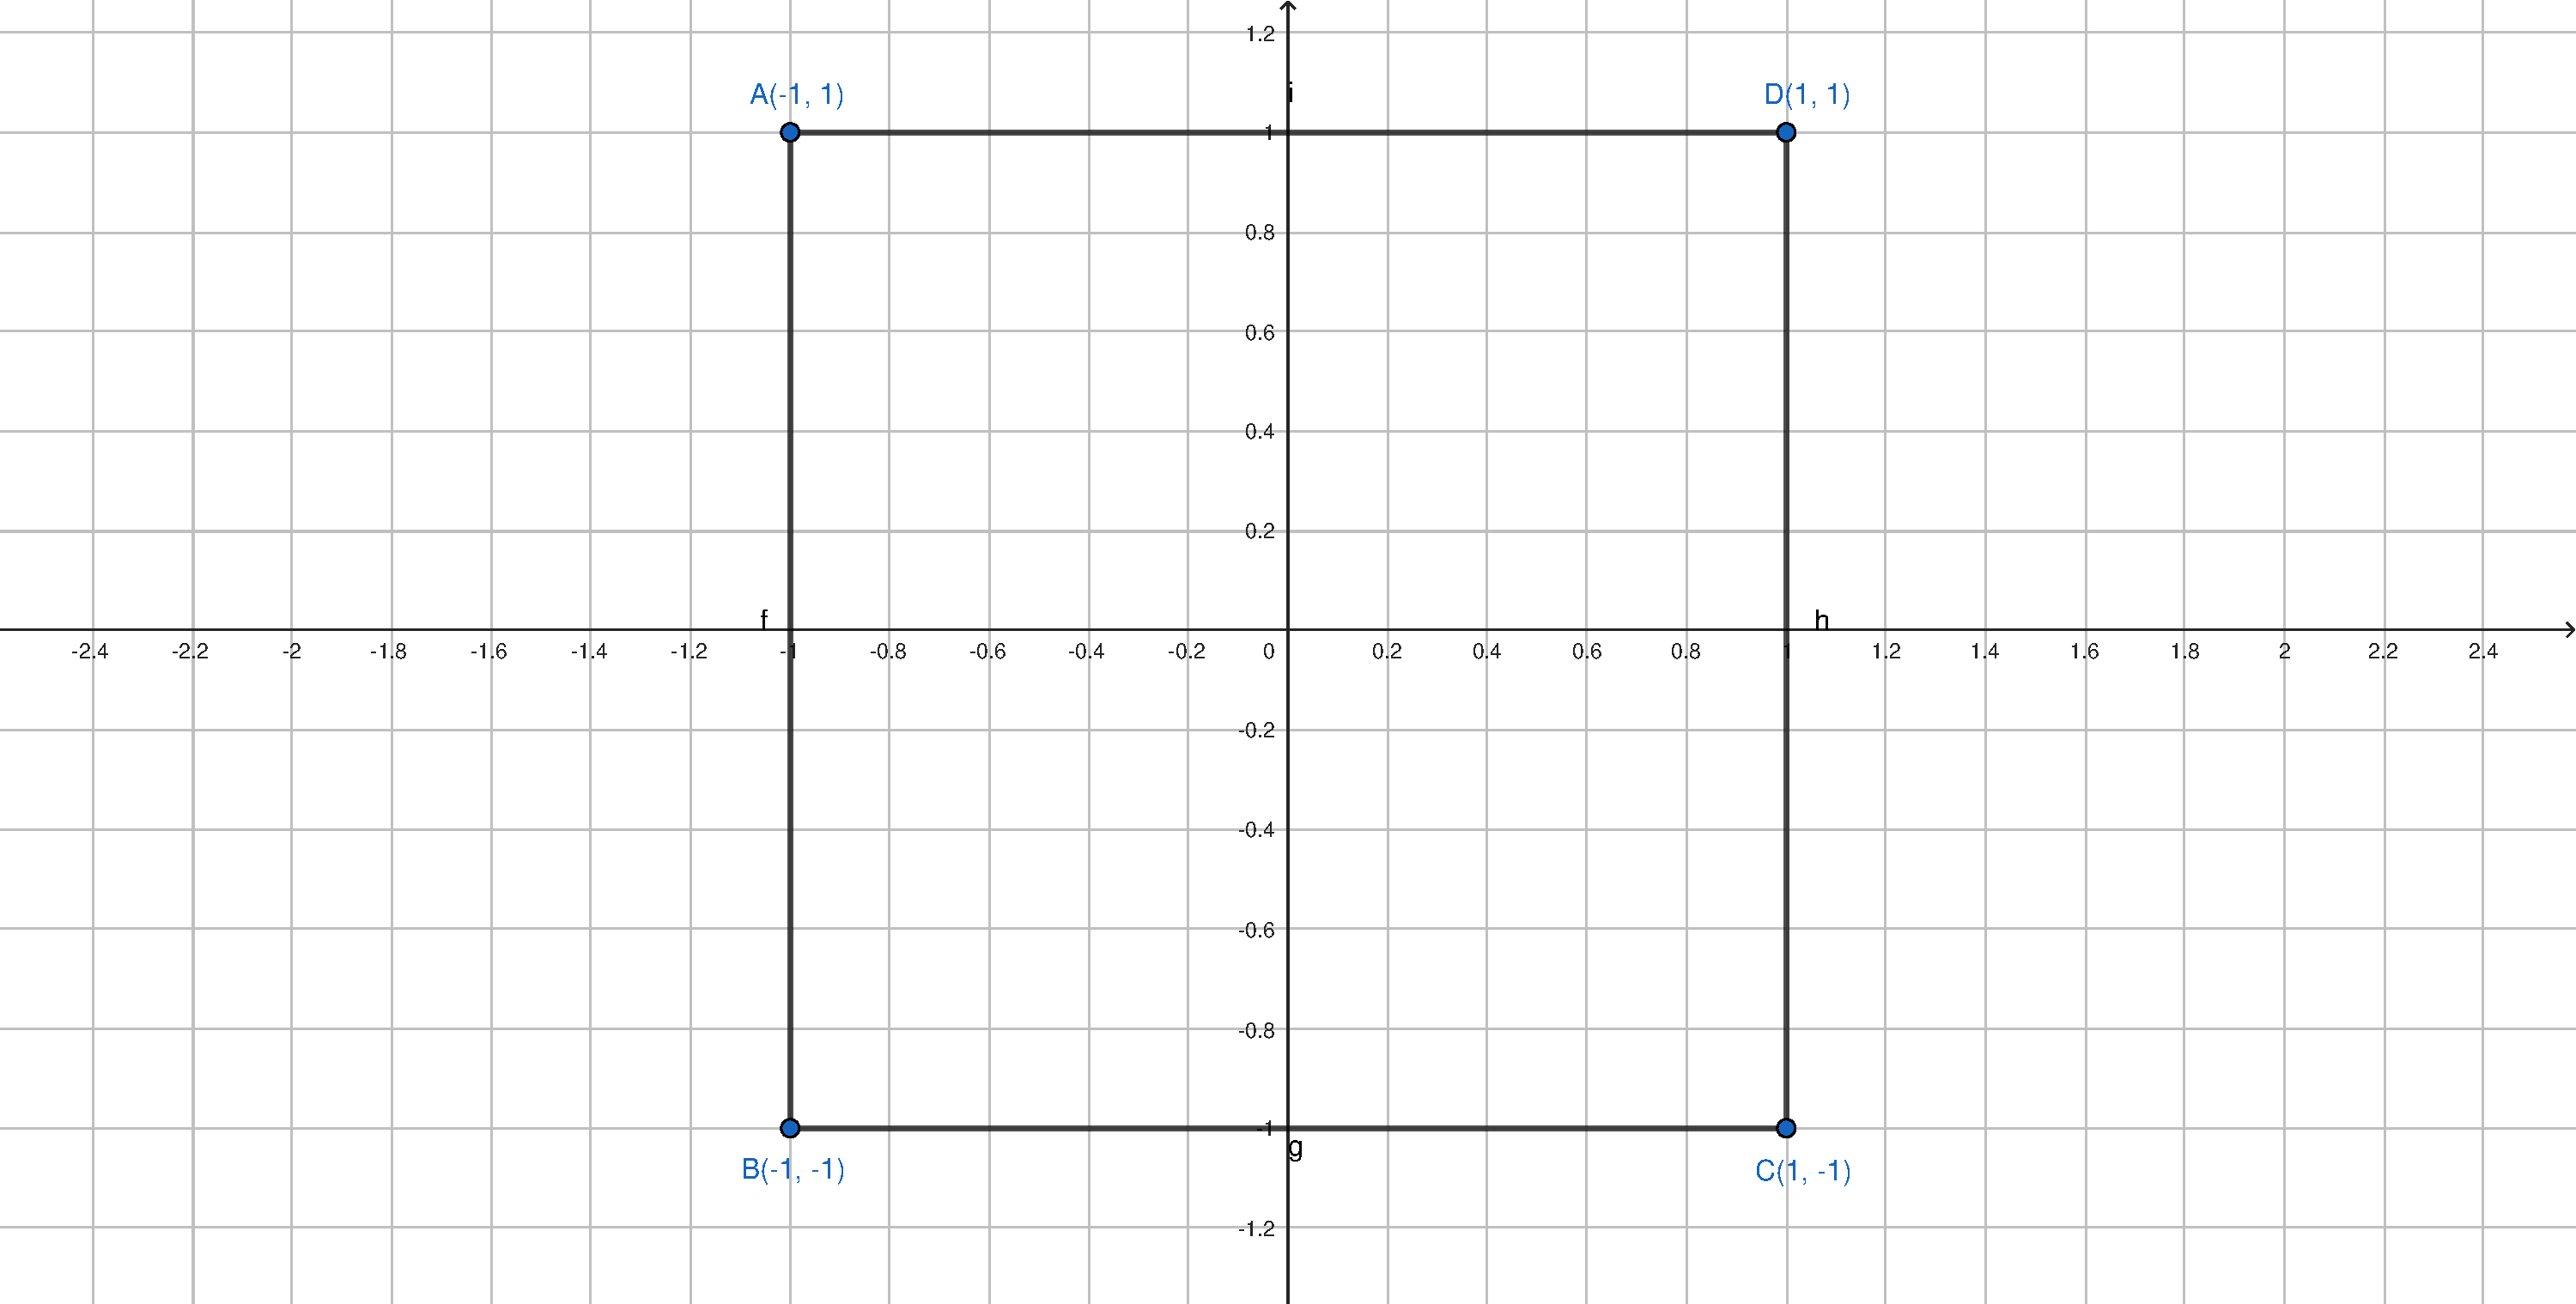
\includegraphics[width=1.5\textwidth]{paths.pdf}
            \end{figure}
    \item (5 points) Are parts (a) and (b) consistent with each other? Why or why not?
    \end{enumerate}

\end{problem}


\newpage
\begin{problem}
    \begin{enumerate}[(a)]
        \item (10 points) State the change of variable theorem. That is, for a change of coordinate
        $\varphi: D \to S$ such that
        \begin{equation*}
            \begin{pmatrix}
                x \\ y
            \end{pmatrix}
            = \varphi(u,v) \,,
        \end{equation*}
        what is the formula for 
        $\iint_S f \, dA$?
    \item (10 points) Evaluate
        \begin{equation*}
            \iint_S xy \, dA
        \end{equation*}
        where $S$ is the disk with radius $2$ and has center at $(0,0)$.
        
\end{enumerate}
\end{problem}



\newpage

\begin{problem}
    A rectangular box with a lid is made from $12 m^2$ of cardboard.
    Find the maximum volume of such a box.

    (Hint: set up a constraint optimization problem for the function $V(x,y,z) = xyz$ 
    and then solve it.)
\end{problem}
%\bibliography{refs}


\end{document}
